\documentclass{article}
\usepackage[utf8]{inputenc}

\title{spettro di radiazione di un corpo nero}
\author{Giulia Cantarini}
\date{Giugno 2020}

\usepackage{amsmath, amsthm}

\usepackage{natbib}
\usepackage{graphicx}
\usepackage[margin=2.0cm]{geometry}

\usepackage{wrapfig}

\usepackage[utf8]{inputenc}
\usepackage[italian]{babel}
\usepackage[T1]{fontenc}
\usepackage{pgfplots}
\theoremstyle{definition}
\newtheorem{defin}{definizione}[section]
\newtheorem{richi}{richiamo}[section]
 

\begin{document}

\maketitle


\section*{Introduzione}
Ogni corpo materiale emette, così come assorbe, radiazioni elettromagnetiche in modo tale da mantenere un equilibrio energetico col sistema esterno.

\begin{defin}{radiazione elettromagnetica}
fenomeno ondulatorio dato dalla concatenazione di campi elettrici e magnetici che trasporta energia sotto forma di luce e calore
\end{defin}
Ogni onda ha una lunghezza d'onda propria, per studiare la radiazione assorbita o emessa da un corpo è dunque necessario individuare lo spettro di quel corpo
\begin{defin}{spettro di emissione di un corpo}
distribuzione che rappresenta l'intensità di irradiazione(o irraggiamento) associata a ciascuna lunghezza d'onda emessa
\end{defin}
Il caso ideale del corpo nero viene utilizzato come modello perché le sue distribuzioni spettrali sono indipendenti dalla composizione chimica e dalle caratteristiche fisico-geometriche del corpo, variando esclusivamente in base alla temperatura. Queste ultime infatti normalmente rendono molto più complesso lo studio in termini scientifici delle capacità di emissione e di assorbimento di un corpo.
Ciò è possibile in quanto il corpo nero, il cui caso può essere approssimato a quello di una cavità opaca con un foro dalle dimensioni molto ridotte rispetto a quelle della cavità, è assorbitore ed emettitore perfetto di radiazioni. Per quanto riguarda i corpi neri il potere assorbente è quindi pari ad 1 (il suo spettro di assorbimento sarà completamente nero) ed il potere emissivo è il medesimo per tutti e dipende solo da T.
\section*{Distribuzione spettrale di un corpo nero}
La distribuzione spettrale dell'intensità delle radiazioni emesse da un corpo nero ha unità di misura pari a \(\frac{W/m^{2}}{m}\) e rappresenta la potenza per unità di superficie emessa per unità di lunghezza d'onda, ovvero l'irraggiamento per unità di lunghezza d'onda. Mentre l'irraggiamento complessivo ha unità di misura \(\frac{W}{m^{2}}\) e coincide con l'area compresa tra la curva e l'asse delle ascisse.\\
\begin{figure}[h!]
    \centering
    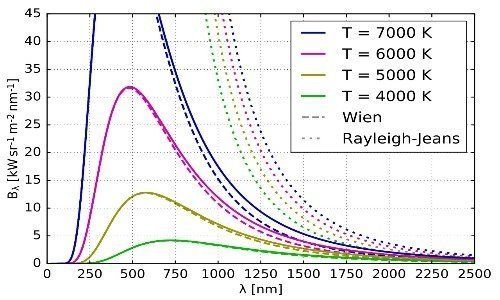
\includegraphics[scale=0.5]{corpo-nero.jpg}
%    \caption{Caption}
    \label{fig:my_label}
\end{figure}
L'irraggiamento di un corpo nero per unità di lunghezza d'onda dipende solo da T e da \(\lambda\):

\begin{equation}
R(\lambda;T) = \frac{2\pi h c^{2}}{\lambda^{5}\left ( e^{\frac{hc}{\lambda kT}}-1\right )}
\end{equation}


dal grafico notiamo che le curve corrispondenti a temperature diverse sono simili; in ognuna di esse si presenta un punto di massimo \(\lambda\) max per il quale l'emissione di radiazioni ha intensità massima (tale lunghezza d'onda determina il tipo di luce che vedo emettere dal corpo).

L'aumento della temperatura determina
\begin{itemize}
\item un aumento dell'energia trasportata per tutte le lunghezze d'onda, e quindi dell'intensità luminosa complessiva. Tale è regolato dalla legge di Stefan-Boltzmann che definisce l'intensità di irraggiamento estesa a tutte le lunghezze d'onda come direttamente proporzionale a T alla quarta
\end{itemize}
\begin{equation}
I(T)=\delta T^{4}     \text{     con  } \delta = 5,67\cdot 10^{-8}\frac{W}{m^{2}K^{4}}
\end{equation}
I(T) è rappresentata dall'area compresa tra la curva e l'asse delle ascisse, ossia \(
I(T) = \int_{0}^{\infty} R(\lambda ; T)d\lambda 
\)
e la sua unità di misura è \(\frac{W}{m^{2}}\) (potenza irraggiata per unità di area del foro di emissione, relativa a una fissata T)

\begin{itemize}
\item una diminuzione della \(\lambda\) max. Lo spostamento delle \(\lambda\) max al variare di T segue un andamento iperbolico rappresentato dalla legge dello spostamento di Wien
\end{itemize}
\begin{equation}
\lambda \text{max}\cdot T = 2,90\cdot 10^{-3}mK
\end{equation}
notiamo che solo i corpi che superano una certa temperatura emettono prevalentemente radiazione nel campo del visibile, e sono quindi "luminosi".
\section*{L'ipotesi di Plank}
Il tentativo di derivare da una interpretazione teorica la distribuzione delle frequenze della radiazione emessa da un corpo nero venne inizialmente messo in atto usufruendo delle conoscenze allora possedute 
\begin{itemize}
\item elettromagnetismo: permette di comprendere, attraverso le leggi di Maxwell, come avviene la propagazione della radiazione elettromagnetica
\item termodinamica: di cui fa parte il principio di equipartizione dell'energia, che stabilisce come è distribuita l'energia nelle varie componenti di un corpo quando questo è portato a temperatura T e si trova in equilibrio termico
\item meccanica: le leggi della dinamica, in particolare quelle che descrivono il moto delle particelle responsabili dell'assorbimento e dell'emissione dell'energia di radiazione
\end{itemize}
Consideriamo un corpo nero in equilibrio termico a temperatura T; quando una radiazione incide sul foro e raggiunge l'interno della cavità, avviene uno scambio continuo di energia tra le pareti della cavità e la radiazione elettromagnetica al suo interno. Tale corpo emetterà una radiazione con le stesse caratteristiche di quella che assorbe. Tale radiazione, secondo le leggi di Maxwell, si comporta come un'onda, la quale è tuttavia vincolata dalle pareti della cavità ed è dunque stazionaria.
\begin{richi}{richiami onde stazionarie}

\par le onde stazionarie sono perturbazioni oscillanti che presentano dei nodi alle estremità in cui si ha ampiezza nulla. In un'onda stazionaria l'ampiezza di oscillazione è solo in funzione della posizione, difatti la funzione d'onda è 
\end{richi}

\begin{equation}
y=A \cos(\frac{2\pi x }{\lambda}) \cos(\omega t)
\end{equation} 
i nodi dell'oscillazione fondamentale si trovano ponendo \(\cos(\frac{2\pi x}{\lambda})=0\)    ovvero    \(\frac{2\pi x}{\lambda } = \pm \frac{\pi }{2}\)      \(x=\pm\frac{\lambda} {4}\)     quindi    \(L=2\frac{\lambda}{4}\)


Le onde stazionarie che si propagano su una lunghezza L possono avere infiniti nodi, l'unica costante è che \(L=n\frac{\lambda }{2}\) con n=0,1,2,...
\par Allo stesso modo le onde elettromagnetiche possono propagarsi con qualunque \(\lambda\) in ogni lunghezza della cavità, più \(\lambda\) è piccola (o n è grande) più il numero di onde possibili si alza e con esso l'energia totale trasmessa agli atomi della cavità dalle stesse. Il problema della visione classica, in cui si erano imbattuti anche Rayleigh e Jeans con la loro formula per la distribuzione spettrale di corpo nero, sussiste proprio a causa di questa energia infinita trasmessa agli atomi che a loro volta dovrebbero emetterne altrettanta; tale fenomeno non può verificarsi.
\par Planck avanzò allora l'ipotesi che gli atomi potessero assorbire solo quantità discrete di energia al momento dell'incidenza con le onde, invece di comportarsi come oscillatori ideali elementari la cui energia è una variabile continua (secondo le leggi classiche della termodinamica e dell'elettromagnetismo, infatti, quando una radiazione colpisce un oggetto i suoi atomi cominciano ad oscillare più rapidamente per via dell'energia acquisita, senza limiti nell'assorbimento).
\begin{richi}{richiami oscillatori armonici}
\par nel caso di una massa m appesa ad una molla che oscilla in un intervallo con ampiezza [-A;+A], l'oscillatore ha energia meccanica costante data dalla somma dell'energia potenziale elastica con quella cinetica, le quali variano trasformandosi continuamente l'una nell'altra
\end{richi}

Emeccanica = Ec + Ep = \(\frac{1}{2} m V^{2} + \frac{1}{2} k x^{2}   \Rightarrow  \frac{1}{2} m A^{2} \omega ^{2}\) e \(\frac{1}{2} k A^{2}\) sono i due modi più semplici di esplicitare E, che notiamo essere direttamente proporzionale alla f al quadrato in quanto:
\begin{align*}
&x(t)=A \cos(\omega t) \text{  legge oraria del moto oscillante}\\ 
&V(t)=-A\omega \sin (\omega t) \text{  derivata prima dello spazio} \rightarrow Vmax=\pm A\omega\\
&a(t)=-A\omega ^{2} \cos(\omega t) = -\omega ^{2} x \text{  derivata prima della V}
\end{align*}
sostituisco a(t) in \(Fe=-kx=ma\) data dalla legge di Hook e dal secondo principio della dinamica. Ottengo \(\omega=\sqrt{\frac{k}{m}}=2\pi f\), ricordiamo che \(E=\frac{1}{2} m A^{2} \omega ^{2}  \Rightarrow \) E dipende dalla frequenza, a sua volta legata alla massa oscillante.\\


Sappiamo che l'atomo oscillatore fissato a temperatura T non può avere energia infinita, ma la sua \(\overline{E}\)=Kb T è data dal principio di equipartizione dell'energia
\begin{defin}{principio di equipartizione dell'energia}
afferma che un oscillatore può assumere, per ognuno dei suoi 2 gradi di libertà, una quantità di energia pari a \(\frac{1}{2}Kb T\).
\end{defin}

In ultima analisi l'ipotesi rivoluzionaria di Planck consiste nel supporre che l'energia possa essere trasmessa esclusivamente per pacchetti discreti, i quali sono tanto più impercettibili quanto più la massa dell'oscillatore è elevata.  Una massa infinitesima come quella dell'atomo determina delle frequenze (vedi relazione sopra) elevate a cui corrispondono salti di energia tanto alti da superare l'energia consentita per l'oscillatore. Esso rimane dunque congelato a quel livello di energia.
Per questo motivo nel grafico dell'irraggiamento complessivo notiamo che più \(\lambda\) tende a 0 più gli atomi faticano a raggiungere il livello di energia corrispondente a quella frequenza e l'intensità di emissione per quella \(\lambda\) diminuisce. 
\begin{equation}
    E=n h f \text{  con n=1,2,3,...}\Rightarrow \text{l'energia di un oscillatore armonico è quantizzata}
\end{equation}


\section*{Il caso limite}
Se l'energia corrispondente a ciascuna f è posta in relazione ad essa attraverso una costante di proporzionalità h molto piccola, i salti energetici risultano impercettibili per un oscillatore macroscopico. Le leggi della fisica classica sono dunque dei casi limite della fisica quantistica per h \(\rightarrow\) 0.
\begin{defin}{principio di corrispondenza}
la teoria dei quanti deve concordare con quella classica entro i limiti nei quali la teoria classica concorda con i dati sperimentali, ovvero quando il numero quantico n diventa molto alto.
\end{defin}
applicazione del principio di corrispondenza nel caso del corpo nero\\

\begin{align*}
&R(\lambda ; T) = \frac{2\pi c^{2}T}{\lambda ^{4}} \qquad\text{equazione ricavata da Rayleigh-Jeans classicamente}\\
&R(\lambda;T) = \frac{2\pi h c^{2}}{\lambda^{5}\left ( e^{\frac{hc}{\lambda kT}}-1\right )} \qquad\text{equazione ricavata da Planck}
\end{align*}
Calcolo \(\lim_{h \rightarrow 0} \frac{2\pi h c^{2}}{\lambda^{5}\left ( e^{\frac{hc}{\lambda kT}}-1\right )}\) ricordando che, per il limite notevole \(\lim_{x\rightarrow 0}\frac{\left ( e^{x}-1\right )}{x}=1\) vale \(\lim_{x\rightarrow 0}\left ( e^{x}-1\right )=x\)\\
considero \(\frac{hc}{\lambda kT}\) come x e scrivo \(\lim_{\frac{hc}{\lambda kT} \rightarrow 0} \frac{2\pi h c^{2}}{\lambda^{5}\left ( e^{\frac{hc}{\lambda kT}}-1\right )} = \frac{2\pi h c^{2}}{\lambda^{5}} \frac{k\lambda T}{hc} = \frac{2\pi c^{2}T}{\lambda ^{4}}\) che corrisponde alla equazione di Rayleigh-Jeans per la distribuzione spettrale.

\newpage
\section*{Studio analitico della distribuzione spettrale}


Traccio un grafico associato ad una temperatura qualsiasi\\

\begin{minipage}{0.4\textwidth}
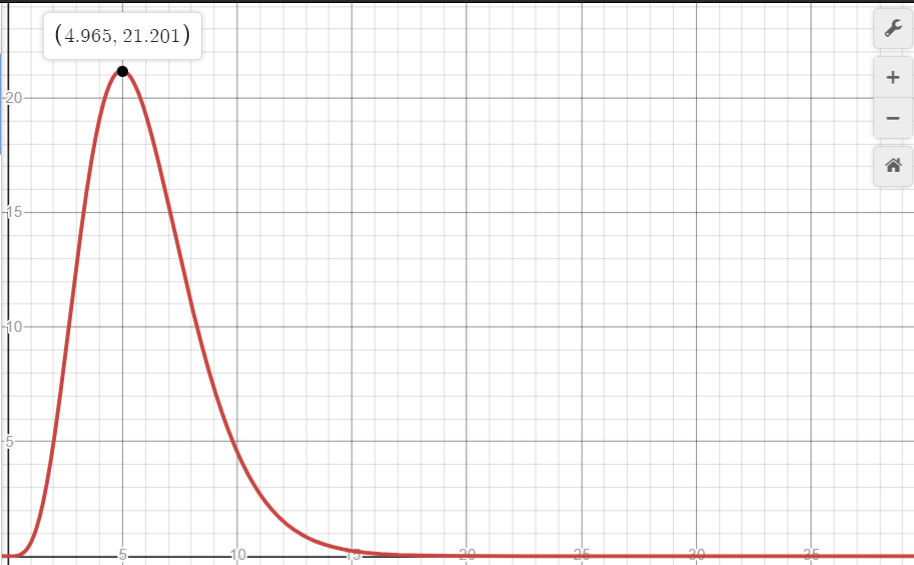
\includegraphics[width=\linewidth]{grafico1.png}
\end{minipage}

fissata una temperatura di 6000K, D:[0;+\(\infty\)]   C:[0;9,93 \(10^{13}\)],
la funzione è continua nel suo dominio e lambda ha un andamento talvolta esponenziale e talvolta come potenza. E' sempre positiva perché lambda è una lunghezza sempre positiva e \(\left (e^{\frac{hc}{\lambda kT}}-1\right )>0\rightarrow \frac{hc}{\lambda kT}>0\) vale sempre
\begin{equation}
\lim_{\lambda \rightarrow 0} R(\lambda ;T)=\frac{2\pi h c^{2}}{0} \cdot \frac{1}{\left (e^{\infty }-1  \right )}=    \infty\cdot 0=\lim_{\lambda \rightarrow 0}\frac{\frac{2\pi h c^{2}}{\lambda ^{5}}}{\left ( e^{\frac{hc}{\lambda kT}}-1\right )}=\frac{\infty}{\infty}=0 \text{    punto di intersezione con y=0 in x=0}
\end{equation}
perché, secondo la gerarchia degli infiniti, date le funzioni
\begin{equation}
\left ( log_{a}x \right )^{\alpha }, x^{\beta }, b^{x} con \alpha ,\beta > 0 e a,b > 1 \text{    per   } x\rightarrow \infty 
\text{   vale, riferendoci agli ordini di infinito, che   }
\left ( log_{a}x \right )^{\alpha }<x^{\beta }<b^{x}
\end{equation}
\begin{equation}
\lim_{\lambda \rightarrow \infty }R(\lambda ;T)=\frac{2\pi h c^{2}}{\infty} \cdot \frac{1}{\left (e^{0 }-1  \right )} =  0\cdot \infty=\lim_{\lambda \rightarrow \infty}\frac{\frac{2\pi h c^{2}}{\lambda ^{5}}}{\left ( e^{\frac{hc}{\lambda kT}}-1\right )}=\frac{0}{0} =\lim_{\lambda \rightarrow \infty }\frac{-10\pi hc^{2}}{\lambda ^{6}\left ( \frac{-hc}{kT\lambda^{2}}e^{\frac{hc}{k\lambda T}} \right )}=\frac{cost}{\infty \cdot 1}=0
\end{equation}
applico il teorema di De l'Hopital, per il quale, se sono soddisfatte alcune ipotesi, vale \(\lim_{x\rightarrow x_{0}}\frac{f(x)}{g(x)}=\lim_{x\rightarrow x_{0}}\frac{f'(x)}{g'(x)}\):  per il numeratore ho applicato la formula per la derivata di una potenza che moltiplica una costante, con il denominatore la derivata di una differenza e poi la derivata di una esponenziale con esponente f(x)\\
ho trovato un asintoto orizzontale y=0.

Ricerco i punti stazionari della funzione ponendo la derivata prima=0, per farlo sostituisco per comodità

\begin{align*}
&x=\frac{h c}{\lambda k T}\rightarrow \lambda =\frac{h c}{x k T} \text{   e ottengo   }
R(\lambda ;T)=\frac{2\pi x^{5}k^{5}T^{5}}{h^{4}c^{3}\left ( e^{x}-1 \right )}=\frac{a x^{5}}{\left ( e^{x}-1 \right )}\\
&R'(\lambda ;T)=\frac{a\left [ 5x^{4}\left ( e^{x}-1 \right )-e^{x}x^{5}\right ]}{\left ( e^{x}-1 \right )^{2}}=0 \Leftrightarrow 5\left ( e^{x}-1 \right )=e^{x}x\Rightarrow \frac{5}{x}=\frac{1}{1-e^{-x}} \qquad
\end{align*}

\par Ho sviluppato la derivata del quoziente e posto \(a = \frac{2\pi k^{5}T5}{h^{4}c^{3}}\). Ora calcolo, utilizzando il metodo di bisezione, il valore approssimato delle radici dell'equazione \(\frac{5}{x}=\frac{1}{1-e^{-x}}\) per le quali la derivata si annulla. Il grafico mi dice che la soluzione è una sola:

\vspace{0.5cm}

\begin{minipage}{0.4\textwidth}
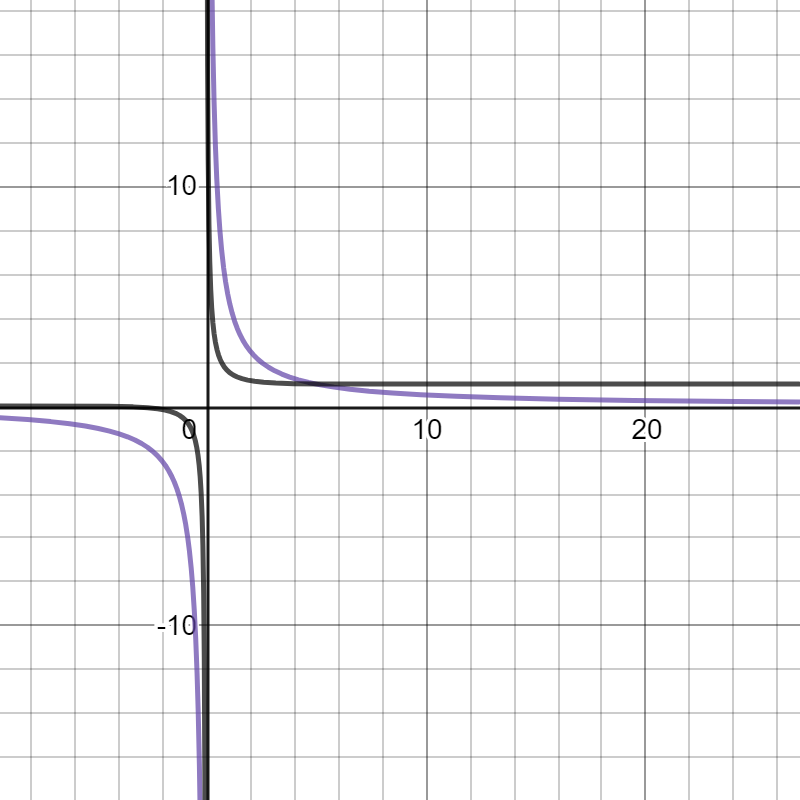
\includegraphics[width=\linewidth]{grafico2.png}
\end{minipage}
\hspace{0.5cm}
\begin{minipage}{0.5\textwidth}
Cerco la soluzione c nell'intervallo [4;6], all'interno del quale si intersecano le funzioni \(\frac{5}{x}\) e \(\frac{1}{1-e^{-x}}\). L'esistenza e l'unicità di tale soluzione è confermata per R'(x)=\(\frac{5}{x}-\frac{1}{1-e^{-x}}\) dai teoremi di esistenza e unicità degli zeri le cui ipotesi sono verificate perché f(4)f(6)<0 e la derivata prima di f(continua e derivabile in [4;6]) non si annulla mai.\\
Procedo con l'approssimazione indicando il punto medio dell'intervallo (un primo valore approssimato della soluzione c), ovvero 5. Ne cerco uno più preciso:\\
\\
M1(5;0): R'(M1)= -0,00678 e R'(4)= 0,231 discordanza -> c è compreso in [4;5] per il teorema dell'esistenza degli zeri\\
M2(4,5;0): R'(M2)= 0,0999 e R'(5)= -0,00678 disc\\
M3(4,75;0): R'(M3)= 0,0439 e R'(5)= -0,00678 disc\\
M4(4,88;0): R'(M4)=0,0169 e R'(5)= -0,00678 disc\\
M5(4,94;0): R'(M5)=0,00494 e R'(5)= -0,00678 disc\\
M6(4,97;0): R'(M6)= -0,000955 e R'(5)= -0,00678 concordanza -> l'intersezione si trova nell'intervallo precedente ossia [4,94;4,97]\\
\end{minipage}

\vspace{0.5cm}

Considerando \(x=\frac{\left ( 4,94+4,97 \right )}{2}=4,955\approx 4,96\) e ricordando che \(\lambda =\frac{h c}{x k T}\), \(\lambda max = 4,84 10^{-7}\); approssimativamente in accordo con la legge dello spostamento di Wien: per T=6000 \(\lambda max= 4,83 10^{-7}\)

La funzione non è monotona nel suo dominio, ma è crescente da 0 fino a tale valore \(\lambda max\); infatti la derivata è positiva solo se \(\frac{5}{x}>\frac{1}{1-e^{-x}}\) e nel grafico vediamo che la funzione viola è maggiore di quella nera solo in quell'intervallo (considero solo lunghezze d'onda positive). R'(x) invece decresce per lunghezze d'onda maggiori di \(\lambda max\).
\section*{Confronto tra la radianza e la sua derivata prima}
Considerata \(\lambda max\) la lunghezza d'onda che corrisponde all'energia KbT minima che un atomo-oscillatore può possedere e quindi emettere a quella T fissata, sappiamo che al diminuire di \(\lambda\) aumenta il salto energetico necessario per acquisire energia superiore e quindi le emissioni per lunghezze d'onda sempre più piccole diminuiscono. All'aumentare di \(\lambda\) il salto è più piccolo ma gli oscillatori tendono a raggiungere l'energia corrispondente alla loro temperatura.
Quindi la funzione R cresce fino a \(\lambda max\) per poi decrescere; dunque nell'intervallo [0;\(4,84 10^{-7}m\)] R' è positiva e si annulla in \(\lambda max\), per poi divenire negativa. La funzione R inoltre presenta due punti di flesso; la derivata seconda, non calcolata perché non espressamente richiesto, quindi si annulla in due punti rispettivamente ai quali la derivata prima varia l'andamento crescente/decrescente. Infine la funzione presenta un asintoto orizzontale che porta la derivata a tendere anch'essa a zero per \(\lambda\) tendente a infinito.
\begin{figure}[h!]
    \centering
    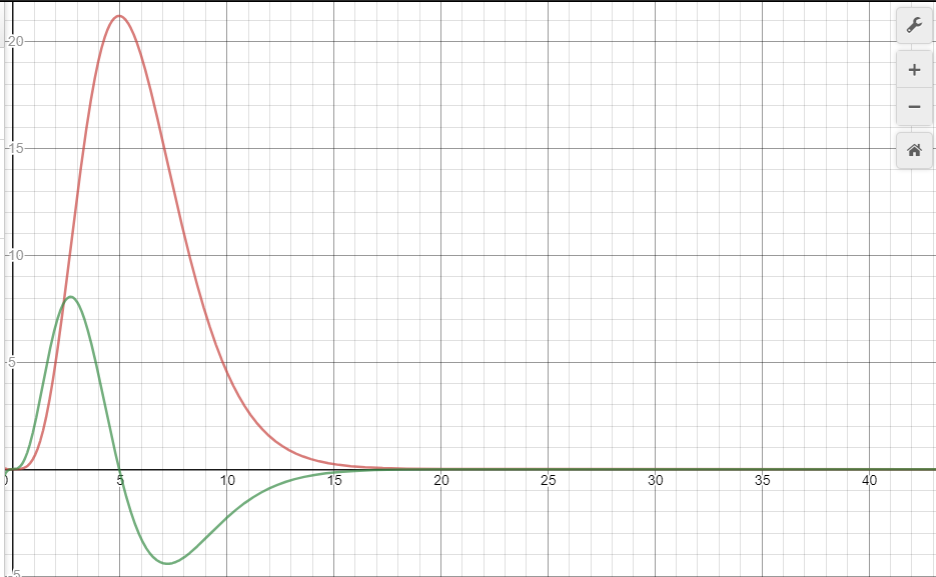
\includegraphics[scale=0.40]{grafico3.png}
%    \caption{Caption}
%    \label{fig:my_label}
\end{figure}



\end{document}
